
%%%%%%%%%%%%%%%%%%%%%%%%%%%%%%%%%%%%%%%%%%%%%%%%%%%%%%%%%%%%%%%%%%%%%%
% njuthesis 示例模板 v1.4.2 2024-11-08
% https://github.com/nju-lug/NJUThesis
%
% 贡献者
% Yu XIONG @atxy-blip   Yichen ZHAO @FengChendian
% Song GAO @myandeg     Chang MA @glatavento
% Yilun SUN @HermitSun  Yinfeng LIN @linyinfeng
% Yukai Chou @Muzimuzhi
%
% 许可证
% LaTeX Project Public License(版本 1.3c 或更高)
%%%%%%%%%%%%%%%%%%%%%%%%%%%%%%%%%%%%%%%%%%%%%%%%%%%%%%%%%%%%%%%%%%%%%%

%---------------------------------------------------------------------
% 一些提升使用体验的小技巧:
%   1. 请务必使用 UTF-8 编码编写和保存本文档
%   2. 请务必使用 XeLaTeX 或 LuaLaTeX 引擎进行编译
%   3. 不保证接口稳定,写作前一定要留意版本号
%   4. 以百分号(%)开头的内容为注释,可以随意删除
%---------------------------------------------------------------------

%---------------------------------------------------------------------
% 请先阅读使用手册:
% http://mirrors.ctan.org/macros/unicodetex/latex/njuthesis/njuthesis.pdf
%---------------------------------------------------------------------

\documentclass[
    % 模板选项(注意右端逗号):
    %
    type = bachelor, % 文档类型,默认为本科生
    % degree = academic|professional,        % 学位类型,默认为学术型
    %
    % nl-cover,   % 是否需要国家图书馆封面,默认关闭
    decl-page,  % 是否需要诚信承诺书或原创性声明,默认关闭
    %
    %   页面模式,详见手册说明
    % draft,                  % 开启草稿模式
    % anonymous,              % 开启盲审模式
    % minimal,                % 开启最小化模式
    %
    %   单双面模式,默认为适合印刷的双面模式
    oneside,                % 单面模式,无空白页
    % twoside,                % 双面模式,每一章从奇数页开始
    %
    %   字体设置,不填写则自动调用系统预装字体,详见手册
    % fontset = win|mac|macoffice|fandol|none,
  ]{njuthesis}

% 模板选项设置,包括个人信息、外观样式等
% 较为冗长且一般不需要反复修改,我们把它放在单独的文件里
% njuthesis 参数设置文件 v1.4.2 2024-11-08

% 一些提醒:
%   1. \njusetup 内部千万不要有空行
%   2. 使用英文半角逗号(,)分隔选项
%   3. 等于号(=)两侧的空格会被忽略
%       3.1. 为避免歧义,请用花括号({})包裹内容
%   4. 本科生无需填写的项目已被特别标注
%   5. 可以尽情删除本注释

% info 类用于录入个人信息
%   带*号的为对应英文字段
\njusetup[info]{
    title = {社交媒体平台网络暴力会伤损害股票市场投资者的获得感吗},
    % 中文题目
    % 直接填写标题就是自动换行
    % 可以使用换行控制符(\\)手动指定换行位置
    %
    title* = {Can Cyberbulling in social media hurt investors's wealth in stock market},
    % 英文题目
    %
    author = {辛昊飞},
    % 作者姓名
    %
    author* = {Xin HaoFei},
    % 作者英文姓名
    % 一般使用拼音
    %
    keywords = {Agent-Based建模,人工股票市场,网络暴力,行为金融,市场效率},
    % 中文关键词列表
    % 使用英文半角逗号(,)分隔
    %
    keywords* = {Agent-Based Modeling,Artificial Stock Market,Cyberbullying,Behaviour Finance,Market Efficiency},
    % 英文关键词
    % 使用英文半角逗号(,)分隔
    %
    grade = {2021},
    % 年级
    %
    student-id = {211275016},
    % 学号或工号
    % 研究生请斟酌大小写字母格式
    % 本模板并不会自动更正大小写
    %
    department = {工程管理学院},
    department* = {School of Management and Engineering},
    % 院系
    %
    major = {金融工程(计算机金融工程实验班)},
    major* = {Financial Engineering},
    % 专业
    %
    % major = {封面专业,摘要专业},
    % 研究生专业型学位可能遇到两处内容不一致的情况
    %
    supervisor = {李心丹,教授},
    supervisor*= {Li XinDan, Professor},
    % 导师全称
    % 使用英文半角逗号(,)分隔中文姓名和职称
    %
    supervisor-ii = {孙煦初, 助理研究员},
    supervisor-ii* = {Sun Xuchu, Research Associate},
    % 第二导师全称
    % 如果确实没有第二导师,不填写即可
    %
    submit-date = {2025-05-20},
    % 提交日期
    % 格式为 yyyy-mm-dd
    % 不填就是编译当天日期
    %
    %
    % 以下均为研究生项
    %
    % degree = {工程硕士},
    % degree* = {Master of Engineering},
    % 覆盖默认学位名称
    %
    field = {物理化学},
    field* = {Physical Chemistry},
    % 研究领域
    %
    chairman = {某某某~教授},
    % 答辩委员会主席
    % 推荐使用波浪号(~)分隔姓名和职称
    %
    reviewer = {
        某某某~教授,
        某某某~教授
    },
    %
    % 答辩委员会成员
    % 一般为四名,使用英文半角逗号(,)分隔
    %
    clc = {O643.12},
    % 中国图书分类号
    %
    udc = {544.4},
    % 国际图书分类号
    %
    secret-level = {公开},
    % 密级
    %
    defend-date = {2022-05-21},
    % 答辩日期
    % 格式为 yyyy-mm-dd
    % 不填就是编译当天日期
    %
    email = {xyz@smail.nju.edu.cn},
    % 电子邮箱地址
    % 只用于出版授权书
    %
    %
    % 以下用于国家图书馆封面
    confer-date = {2022-05-22},
    % 学位授予日期
    %
    bottom-date = {2022-05-23},
    % 封面底部日期
    %
    supervisor-contact = {
        南京大学~
        江苏省南京市栖霞区仙林大道163号
    }
    % 导师联系方式
}

% bib 类用于参考文献设置
\njusetup[bib]{
    style = author-year,
    % 参考文献样式
    % 默认为顺序编码制(numeric)
    % 可选著者-出版年制(author-year)
    %
    resource = {references.bib},
    % 参考文献数据源
    % 需要带扩展名的完整文件名
    % 可使用逗号分隔多个文件
    % 此条等效于 \addbibresource 命令
    %
    option = {
        gbnamefmt = lowercase,
        % 使用仅首字母大写的姓名
        % refsection = chapter,
        % 将参考文献表置于每章后
        % sorting = nyt,
        % 按姓名、年份、标题排序
        labelnumber = true,
        % 启用编号
        % defernumbers = false
        % 延迟编号,确保编号连续
    }
    % 额外的 biblatex 宏包选项
}

% image 类用于载入外置的图片
\njusetup[image]{
    % path = {{./figure/}{./image/}},
    % 图片搜索路径
    %
    % nju-emblem = {nju-emblem},
    nju-name = {nju-name},
    % 校徽和校名图片路径
    % 建议使用 PDF 格式的矢量图
    % 使用外置图片有助于减少编译时间
    % 空置时会自动使用 njuvisual 宏包绘制
    %
    nju-emblem = {nju-emblem-purple},
    % nju-name = {nju-name-purple},
    % 替换为紫色版本
    % 这个选项只能填写一次
    % 切换时要注释掉上方的黑色版本
}

% abstract 类用于设置摘要样式
\njusetup[abstract]{
    toc-entry = false,
    % 摘要是否显示在目录条目中
    %
    % underline = false,
    % 研究生英文摘要页条目内容是否添加下划线
    %
    % title-style = strict|centered|natural
    % 研究生摘要标题样式,详见手册
}

% 目录自身是否显示在目录条目中
\njusetup{
    tableofcontents/toc-entry = true,
    listoffigures/toc-entry   = true,
    listoftables/toc-entry    = true,
}

% 为目录中的章标题添加引导线
\njusetup[tableofcontents/dotline]{chapter}

% math 类用于设置数学符号样式,功能详见手册
\njusetup[math]{
    % style              = TeX|ISO|GB,
    % 整体风格,缺省值为国标(GB)
    % 相当于自动设置以下若干项
    %
    % integral           = upright|slanted,
    % integral-limits    = true|false,
    % less-than-or-equal = slanted|horizontal,
    % math-ellipsis      = centered|lower,
    % partial            = upright|italic,
    % real-part          = roman|fraktur,
    % vector             = boldfont|arrow,
    % uppercase-greek    = upright|italic
}

% theorem 类用于设置定理类环境样式,功能详见手册
\njusetup[theorem]{
    % define,
    % 默认创建内置的七种定理环境
    %
    % style         = remark,
    % header-font   = \sffamily \bfseries,
    % body-font     = \normalfont,
    % qed-symbol    = \ensuremath { \male },
    % counter       = section,
    % share-counter = true,
    % type          = {...}
    % 以上设置项在重新调用 theorem/define 后生效
}

% footnote 类用于设置脚注样式,功能详见手册
\njusetup[footnote]{
  % style = pifont|circled,
  % 使用圈码编号
  %
  % hang = false,
  % 不使用悬挂缩进
}

% 页眉页脚内容设置
\njusetup{
  % header/content = {
  %     {OR}{\thepage},{OL}{\rightmark},
  %     {EL}{\thepage},{ER}{\leftmark}
  %   },
  % 页眉设置,详见手册
  % 奇数页页眉:左侧章名,右侧页码
  % 偶数页页眉:左侧页码,右侧节名
  %
  % footer/content = {}
}

% 页眉页脚的字体样式
% \njusetformat{header}{\small\kaishu}
% \njusetformat{footer}{}

% 在盲审模式下隐藏学校信息
% \njusetup{anonymous-mode/no-nju}

% 一些灵活调整
% \njusetname{type}{本科毕业设计}                 % 我做的是毕业设计
% \njusetname{notation}{术语表}                   % 更改符号表名称
% \njusetlength{crulewd}{240pt}                   % 加长封面页下划线
% \njusetformat{tabular}{\zihao{-4}\bfseries}     % 修改表格环境的字号
% \EditInstance{nju}{u/cover/emblem-img}{align=l} % 左对齐的本科生封面校徽


% 自行载入所需宏包
\usepackage{subcaption} % 嵌套小幅图像,比 subfig 和 subfigure 更新更好
\usepackage{graphicx}
\usepackage{booktabs}   % for three-line table
\usepackage{caption}    % for adjusting table captions
\usepackage{booktabs}
\usepackage{tabularx}
\usepackage{threeparttable}
% \usepackage{siunitx} % 标准单位符号
% \usepackage{physics} % 物理百宝箱
% \usepackage[version=4]{mhchem} % 绘制分子式
% \usepackage{listings} % 展示代码
% \usepackage{algorithm,algorithmic} % 展示算法伪代码

% 在导言区随意定制所需命令
% \DeclareMathOperator{\spn}{span}
% \NewDocumentCommand\mathbi{m}{\textbf{\em #1}}

% 开始编写论文
\begin{document}

%---------------------------------------------------------------------
%	封面、摘要、前言和目录
%---------------------------------------------------------------------

% 生成封面页
\maketitle

% 模板默认使用 \flushbottom,即底部平齐
% 效果更好,但可能出现 underfull \vbox 信息
% 以下命令用于抑制这些信息
\raggedbottom

\begin{abstract}
随着社交媒体在投资者行为中的影响日益增强,网络暴力作为一种极端负面情绪表达方式,其对金融市场系统性风险的潜在影响值得深入探讨。本文基于 Agent-Based 建模方法,构建融合社交传播机制与行为金融模型的人工股票市场系统,模拟网络暴力在社交网络中的扩散如何影响投资者行为决策,并进一步扰动市场价格与财富分布结构。
模型中引入攻击者、受害者与旁观者角色,通过攻击传播、情绪感染与行为反馈构建“情绪—行为—市场”闭环机制。市场结构采用连续双边报价(CDA)机制,投资者基于多维信号进行交易决策,网络暴力对其情绪偏差与参与概率产生动态干预。
通过多组仿真实验,本文系统分析了网络暴力机制对个体行为路径、群体财富演化以及市场效率的扰动效应。结果显示:网络暴力显著降低了散户交易活跃度与终期财富水平,造成群体内财富差距扩大;同时加剧了价格波动、提高了交易摩擦成本,并削弱了市场价格发现能力。
本文研究为理解社交媒体情绪传播如何通过行为反馈机制传导至市场系统提供了建模框架,也为未来建立金融情绪监管预警机制提供理论依据。

\end{abstract}

\begin{abstract*}
As social media increasingly shapes investor sentiment and decision-making, cyberbullying—an extreme form of negative emotional expression—has emerged as a potential source of systemic risk in financial markets. This study develops an Agent-Based artificial stock market model that integrates a social contagion mechanism to examine how the diffusion of cyberbullying through investor networks impacts individual trading behavior and, ultimately, market dynamics.
The model incorporates roles such as attackers, victims, and bystanders, and simulates a feedback loop among emotional contagion, behavioral responses, and market outcomes. A continuous double auction (CDA) mechanism governs market transactions, where heterogeneous agents make trading decisions based on fundamental, technical, and noise signals. The propagation of cyberbullying alters their emotional bias and participation probability over time.
Through a series of Monte Carlo simulations, the study quantitatively assesses the impact of cyberbullying on trading frequency, wealth distribution, price volatility, market liquidity, and informational efficiency. Results show that cyberbullying significantly reduces retail investor participation and terminal wealth, widens intra-group wealth inequality, increases market volatility, raises transaction costs, and weakens the market's ability to reflect fundamental values.
This research provides a novel framework for modeling the behavioral transmission of extreme social emotions into market-level disruptions and offers theoretical insights for future design of financial emotion monitoring and regulatory mechanisms.

\end{abstract*}

% 生成目录
\tableofcontents
% 生成图片清单
\listoffigures
% 生成表格清单
\listoftables

%---------------------------------------------------------------------
%	正文部分
%---------------------------------------------------------------------
\mainmatter

% 符号表
% 语法与 description 环境一致
% 两个可选参数依次为说明区域宽度、符号区域宽度
% 带星号的符号表(notation*)不会插入目录
% \begin{notation}[10cm]
%   \item[DFT] 密度泛函理论 (Density functional theory)
%   \item[DMRG] 密度矩阵重正化群 (Density-Matrix Reformation-Group)
% \end{notation}

% 建议将论文内容拆分为多个文件
% 即新建一个 chapters 文件夹
% 把每一章的内容单独放入一个 .tex 文件
% 然后在这里用 \include 导入,例如
%   \include{chapters/introduction}
%   \include{chapters/environments}



\chapter{引言}
这里是引言

\chapter{文献综述}
这里是文献综述
\chapter{模型设定}

\section{模型总体框架}

本研究构建了一个集成社交传播机制与行为金融模型的人工股票市场系统,旨在模拟网络暴力这一极端情绪事件如何通过社交网络影响投资者行为,并进一步扰动市场运行机制。整体模型以Agent-Based建模为基础,包含投资者行为模块、市场交易结构模块、网络暴力传播模块和实验分析模块四大核心组成部分,四者在系统中相互耦合,构成“情绪—行为—市场”闭环反馈结构。

在该系统中,投资者被建模为具有异质偏好、有限理性与社交关系的自主Agent,分为机构投资者与散户两类。两类Agent均可基于基本面预期、趋势信号与随机扰动做出交易决策,但在行为风格与受情绪影响程度上存在显著差异,特别是散户更易受到网络暴力影响而表现出沉默或激进等行为偏差。

市场交易结构采用连续双边报价(Continuous Double Auction, CDA)机制,通过订单簿系统撮合市价单与限价单形成成交价格。基础资产价格由布朗运动驱动,模拟市场的外部波动环境。所有Agent的交易意愿以订单形式提交至市场,经过撮合成交,最终影响市场价格演化与财富流动路径。

网络暴力传播模块在散户投资者之间建立社交网络,模拟在社交媒体语境下攻击性言论的传播过程。该模块引入攻击者、受害者、旁观者三类角色转化机制,并设计了情绪感染(正反馈)与系统治理(负反馈)机制。具体传播过程遵循以下逻辑:攻击者选择邻居中的异见者进行言语攻击,受害者若暴露程度超过阈值则转为沉默或反击者,同时系统可通过举报、监管干预或个体心理韧性成长抑制传播范围。

实验分析模块用于对模型结果进行系统分析,主要从两个角度进行分析:一是投资者群体的财富状态变化,二是市场的总体状态(如流动性、波动性等)。该模块通过对两类投资者(散户与机构)财富变化的追踪,分析网络暴力情绪如何影响投资者的财富分布;同时,分析市场的流动性、波动率等指标,探讨网络暴力是否对市场质量产生显著影响。实验分析模块通过对比不同情境下的结果,验证网络暴力对市场的实际影响。

模型整体运行流程如下:在每个仿真时间步,市场随机激活部分投资者进行决策;网络暴力模块并行更新网络暴力状态;投资者依据当前情绪状态、策略参数与市场信息做出交易决策;订单经由市场结构撮合成交;价格、资产与情绪状态更新,进入下一个时间步。通过多轮模拟与对比实验,可以观察网络暴力机制在投资者行为、市场稳定性与财富演化中的影响路径。


\begin{figure}[h]
    \centering
    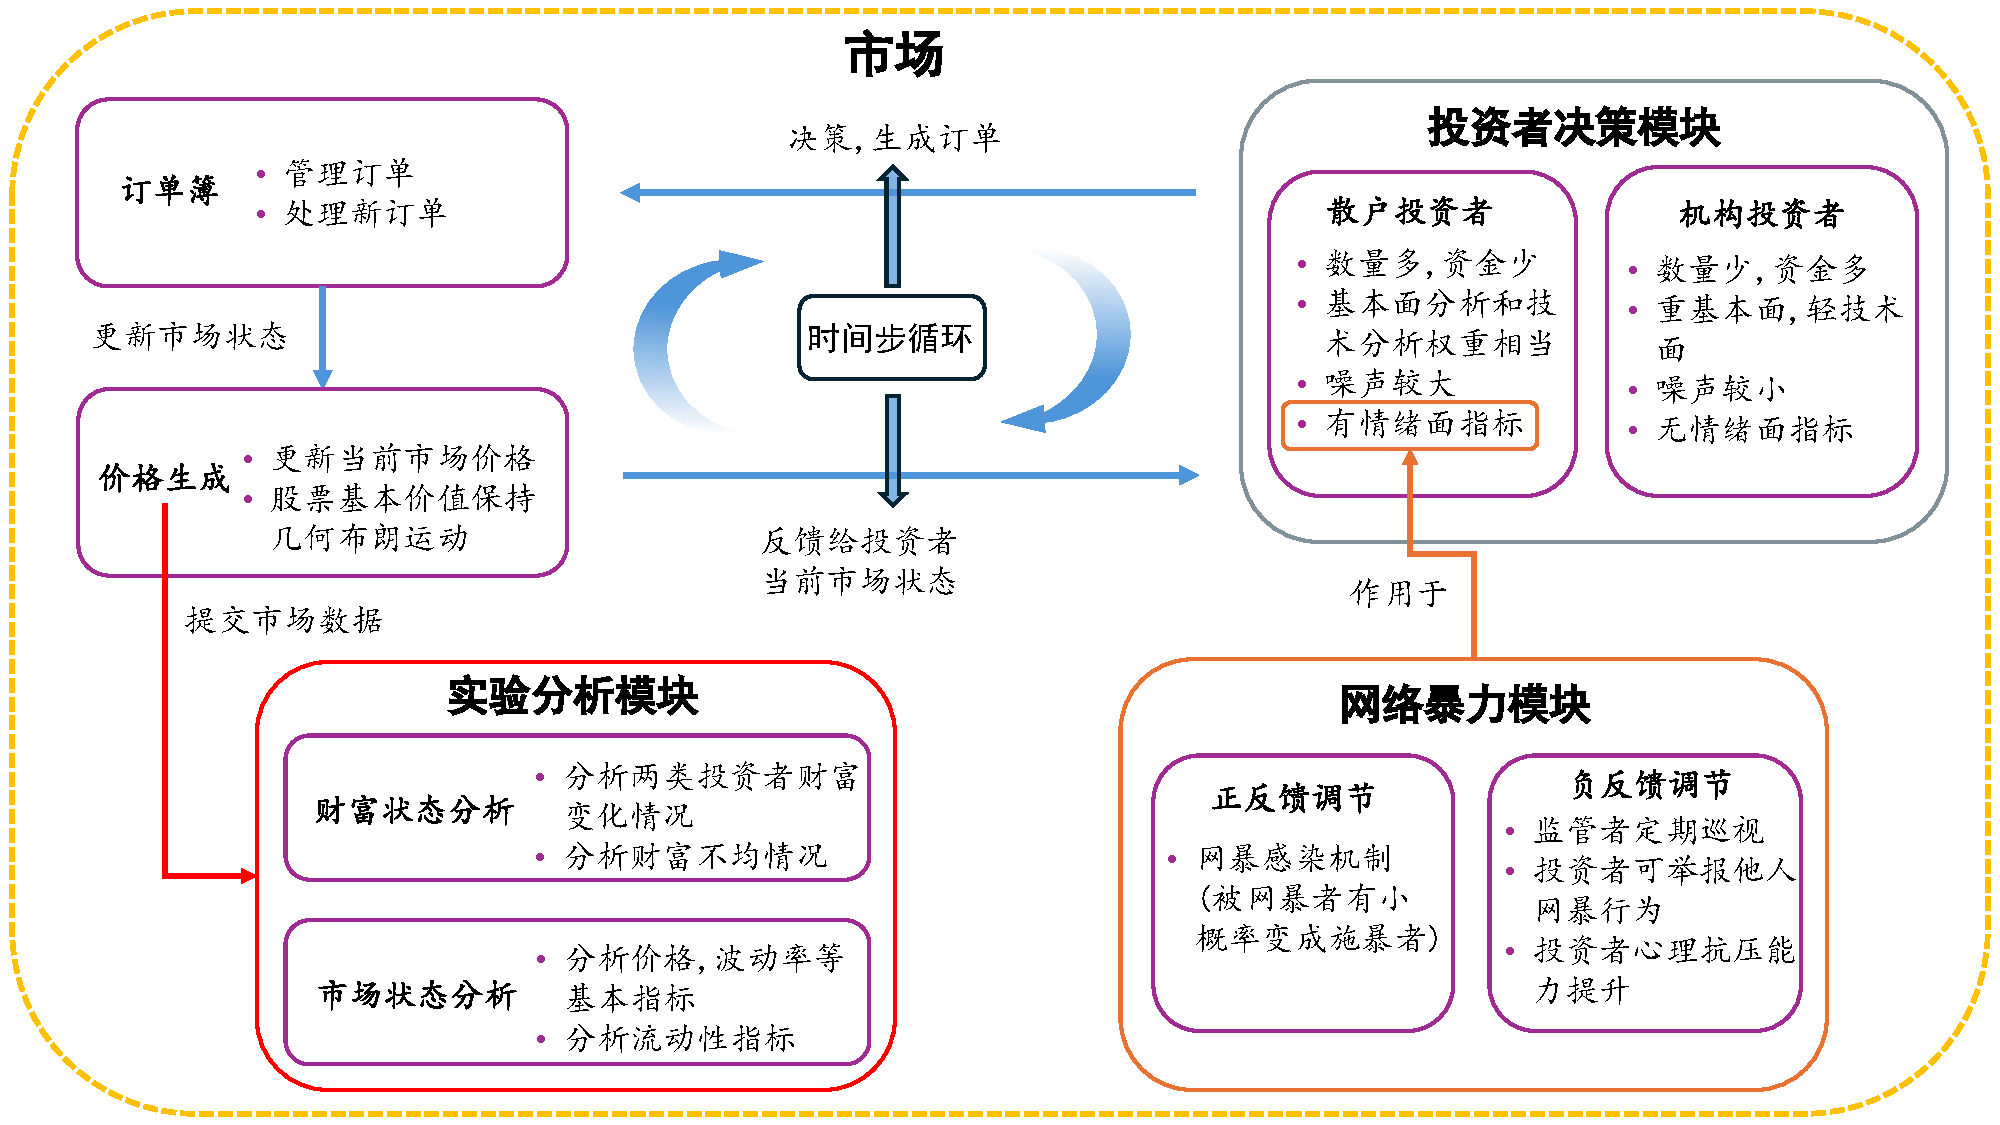
\includegraphics[width=0.8\textwidth]{image/3-1_structure.pdf}
    \caption{模型整体架构}
    \label{fig:architecture}
\end{figure}

图\ref{fig:architecture} 展示了模型的总体结构框架,四个核心子系统通过状态变量与行为函数实现交互,形成多层次、跨模块的系统性耦合。








\section{市场运行机制建模}

本部分模拟了股票市场中的运行机制,特别是订单簿管理、订单匹配以及价格生成过程。本部分将首先讨论订单和订单簿的功能与实现,随后分析市场如何通过订单簿撮合机制生成价格并更新市场状态。

\subsection{订单与订单簿}


市场交易通过订单簿(Order Book)进行管理,订单簿包含市场上所有的买单和卖单,按照价格优先和时间优先的规则进行排列,并通过撮合机制完成交易。在本模型中,投资者可以提交两种类型的订单:市价单(Market Order)和限价单(Limit Order)。

市价单是指投资者希望以市场上当前最优价格立即成交的订单,买单市价单与当前最优卖单匹配,卖单市价单与当前最优买单匹配。限价单则是投资者愿意在特定价格或更好价格下买入或卖出资产的订单。限价单会根据价格优先和时间优先的规则排队,价格优先确保更高的买单和更低的卖单优先成交,时间优先则确保在价格相同的情况下,先提交的订单优先成交。

限价单的提交和撮合过程如下:

1. 买单限价单:在订单簿中,买单限价单按价格从高到低排列。只有当卖单的价格满足买单的价格时,买单才能成交。若价格相同,按时间优先规则进行撮合。

2. 卖单限价单:卖单限价单按价格从低到高排列,买单的价格需要等于或高于卖单的价格才会发生成交。若价格相同,按照提交时间优先。

限价单的核心是它为市场提供了深度,当市场价格变动时,挂单价格会进行相应的调整。只有当市场价格到达某个限价单的价格时,订单才会被执行。

另一方面,市价单与限价单的关系较为复杂,市价单会根据当前订单簿中的最优卖单(对于买单市价单)或最优买单(对于卖单市价单)立即执行。市价单的优先性使其能够快速成交,而限价单则在价格条件不满足时等待成交。若市价单的数量大于市场中最优对手单的数量,未成交的部分会转为限价单,继续在订单簿中等待匹配。

市场中的买单和卖单队列由订单簿进行管理。订单簿通过使用堆(heap)数据结构实现对订单的优先级排序。买单按价格从高到低排序,卖单按价格从低到高排序,确保买卖双方能够根据最优价格进行交易,若价格相同则按订单提交顺序先后排列。


表 \ref{tab:buy_orderbook} 展示了一个典型的买单订单簿示意表,其中包括了买单的订单编号、交易者ID、买入数量、价格、时间戳和订单状态等信息。



\begin{table}[htbp]
    \renewcommand{\arraystretch}{1.5} % 行距调整
    \centering
    \begin{tabular}{@{} >{\centering\arraybackslash}p{2.2cm}
                    >{\centering\arraybackslash}p{2.2cm}
                    >{\centering\arraybackslash}p{2.2cm}
                    >{\centering\arraybackslash}p{2.2cm}
                    >{\centering\arraybackslash}p{2.2cm}
                    >{\centering\arraybackslash}p{2.2cm} @{}}
    \toprule\toprule
    订单编号 & 交易者ID & 买入数量 & 价格 & 时间戳 & 订单状态 \\
    \midrule
    1 & 101 & 100 & 99.95 & 1 & 待处理 \\
    2 & 102 & 200 & 99.90 & 2 & 待处理 \\
    3 & 103 & 150 & 99.85 & 3 & 已成交 \\
    4 & 104 & 100 & 99.80 & 4 & 待处理 \\
    5 & 105 & 50  & 99.75 & 5 & 已取消 \\
    \bottomrule\bottomrule
    \end{tabular}
    
    \vspace{1em}
    
    \caption{买单订单簿示意表}
    \label{tab:buy_orderbook}
    \end{table}
    

在实际市场中,订单簿会随时间的推移动态变化,特别是当市场价格波动时,投资者提交的限价单会被重新排序,市价单则根据当前市场价格立即成交。每个时间步,模型会根据最新的市场状态和订单簿情况进行更新,形成价格和市场行为的反馈循环。





\subsection{价格生成机制与市场状态更新}

在本模型中,基础价格由几何布朗运动(Geometric Brownian Motion, GBM)生成,而市场价格则通过市场中的订单簿和交易活动动态生成。
基础价格反映了市场资产的长期趋势和短期波动,而市场价格则是由市场参与者的交易行为和订单簿状况决定的。基础价格和市场价格的相互作用是市场价格动态更新的核心。

1. 基础价格生成

基础价格代表股票的内在价值,其生成依赖于几何布朗运动模型,这是金融市场中常用的价格生成模型。几何布朗运动模型的价格更新公式如下:

\begin{equation}
    p_{t+1}^{f} = p_t^{f} \exp\left( \mu \Delta t + \sigma \epsilon_t \sqrt{\Delta t} \right)
\end{equation}

其中,\( p_{t}^{f} \) 是当前基础价格,\( \mu \) 是漂移项,表示资产的长期趋势,\( \sigma \) 是波动率,表示价格的波动幅度,\( \epsilon_t \) 是标准正态分布的随机扰动项,\(\Delta t\) 是时间步长。

几何布朗运动能够模拟市场中常见的随机波动,反映资产价格的随机性和市场的不确定性。基础价格是市场中的理论价格,它不直接反映交易者的决策和市场供需情况,而是一个由宏观因素和市场波动性驱动的参考价格, 在本模型中是交易者进行基本面分析时的重要参照。

2. 市场价格生成

市场价格是由市场中的买单和卖单通过订单簿的撮合机制决定的。每个市场时间步,投资者通过市价单或限价单提交订单,市场则根据最优买单和最优卖单的价格进行撮合。当买单价格大于或等于卖单的最优价格时,订单会成交,成交价格即为市场价格。
如果在某一时间步没有成交,则市场价格将根据当前最优买单和最优卖单的价格更新,具体公式如下:

\begin{equation}
    \text{Market Price} = 
    \begin{cases} 
    \text{last\_price} & \text{如果上一时间步有交易发生} \\
    \frac{\text{best\_bid} + \text{best\_ask}}{2} & \text{如果上一时间步没有交易发生}
    \end{cases}
\end{equation}
在市场价格的生成过程中,市价单和限价单之间的相互作用起到了关键作用。市价单是根据当前市场最优对手单立即成交的订单,而限价单则需要在特定的价格范围内等待成交。市价单的成交价格通常会成为市场的最新价格,反映了市场供需的实时状况。





3. 市场状态更新

市场价格更新的基本过程如下:

- 市价单成交:市价买单会与当前最优卖单匹配,而市价卖单会与当前最优买单匹配。当市价单和限价单匹配时,成交价格即为最优买单或卖单的价格。
   
- 订单簿更新:每次成交后,订单簿中的相应订单会被移除,剩余的订单根据价格和时间优先规则重新排列。如果价格发生变化,订单簿将更新,确保挂单的顺序正确。

- 市场价格更新:市场成交价格会被用作当前市场的参考价格,并更新市场价格。通过对成交价格的跟踪,市场价格会反映出当前交易者的行为和市场的供需状况。

市场状态的更新不仅仅是价格的变化,还包括市场的流动性、深度和交易量等因素。在每个时间步,市场的流动性和深度都会随着订单簿的变化而更新。
流动性反映了市场能够在不显著影响价格的情况下吸纳大规模交易的能力,而市场深度则表示在特定档位区间内存在的买单和卖单的数量。

市场的买卖价差(Bid-Ask Spread)可以通过以下公式计算:

\begin{equation}
    \text{Bid-Ask Spread} = \text{best\_ask} - \text{best\_bid}
\end{equation}

市场的深度表示市场中各个价格级别的买单和卖单的总数量。市场深度可以通过以下公式进行计算:

\begin{equation}
    \text{Market Depth} = \sum_{i=1}^{n} (\text{buy\_quantity}_i + \text{sell\_quantity}_i)
\end{equation}

其中,\( \text{buy\_quantity}_i \) 和 \( \text{sell\_quantity}_i \) 分别表示在档位 \( i \) 上的买单和卖单数量,\( n \)代表盘口档数(一般为5档)。
市场深度可以反映市场的流动性,即在不显著影响价格的情况下能够吸纳的订单量。





\section{投资者决策建模}


在本模型中,投资者是市场不可或缺的一部分,他们进入市场,根据当前的市场状态与自身的决策逻辑,决定是否提交订单、提交何种类型的订单(买入或卖出)、订单数量、价格和类型等。
投资者被划分为两类:散户(Retail Trader)和机构(Institutional Trader)。这两类交易者共享一套基本的交易框架,但在权重参数与行为偏好方面存在差异,具体将在后续小节中展开。

\subsection{价格预期与交易意愿}
\label{subsec:price expectation}

投资者进入市场时,会基于当前市场状态构造未来一个投资期 \(\tau^i\) 内的价格预期,并据此计算预期收益率。参照\textcite{chiarella2009impact}的做法,所有投资者的预期收益率均由三类成分组成:基本面驱动、趋势跟随以及随机噪声:

\begin{equation}
    \hat{r}_{t,t+\tau^i}^i = 
    \frac{1}{g_1^i + g_2^i + g_e^i + n^i } 
    \left[
    \underbrace{g_1^i \cdot \frac{1}{\tau_f} \ln\left(\frac{p_t^f}{p_t}\right)}_{\text{基本面}} 
    + \underbrace{g_2^i \cdot \bar{r}_t^i}_{\text{技术面}} 
    + \underbrace{g_e^i \cdot \eta_t^i}_{\text{情绪偏差}}
    + \underbrace{n^i \cdot \epsilon_t}_{\text{噪音}} 
    \right]
    \end{equation}
    其中:
    \begin{itemize}
      \item \( p_t \) 为当前市场价格,\( p_t^f \) 为基础价格;
      \item \( \bar{r}_t^i \) 表示投资者 \(i\) 近期观察到的平均收益率,反映其对趋势的感知;
      \item \( \epsilon_t \sim \mathcal{N}(0, \sigma^2) \) 为高斯白噪音;
      \item \( \eta_t^i \) 为投资者 \(i\) 在时间 \(t\) 的情绪偏差,仅对散户设定有效;
      \item \( g_1^i, g_2^i, n^i, g_e^i \) 分别为基本面、技术面、噪音与情绪权重,具体初始化如下。
    \end{itemize}

    基于上述预期收益率,投资者可推导出其未来期望的交易价格:

\begin{equation}
\widehat{p}_{t+\tau^i}^i = p_t \cdot \exp\left( \tau^i \cdot \widehat{r}_{t,t+\tau^i}^i \right)
\label{eq:expected_price}
\end{equation}

其中,\( p_t \) 表示当前市场价格,\( \tau^i \) 是投资者的投资期。该预期价格 \( \widehat{p}_{t+\tau^i}^i \) 也被记作 \( p^* \),在后续订单类型判断中作为关键参照值使用。

值得注意的是,本模型中投资者的行为偏好权重 \(g_1^i\)、\(g_2^i\)、\(n^i\) 以及情绪项权重 \(w_e^i\) 并非设为固定值,而是使用对数正态分布初始化,使得交易者在基本面、技术面、噪音和情绪感知上的敏感度具有异质性:

\begin{equation}
    \begin{aligned}
    g_1^i &\sim \text{Lognormal}(\mu_1, \sigma) \\
    g_2^i &\sim \text{Lognormal}(\mu_2, \sigma) \\
    g_3^i &\sim \text{Lognormal}(\mu_3, \sigma) \\
    n^i   &\sim \text{Lognormal}(\mu_{n}, \sigma)
    \end{aligned}
\end{equation}
    

上述参数的均值 \(\mu_k\) 根据交易者类型(散户或机构)分别设置,标准差 \(\sigma\) 为共享值。
与\textcite{chiarella2009impact}采用的指数分布不同,对数正态分布在本模型中更能表达多数权重集中于中低值、少数极端行为交易者存在的长尾结构。这种设定有助于捕捉市场中“沉默多数”与“极端交易者”共存的现象,从而增强模拟系统的真实感。




\subsection{是否交易与交易方向}
\label{subsec:trade direction}

投资者会将期望价格与当前市场价格 \( p_t \) 做对比,计算价格偏离程度:

\begin{equation}
    \delta_t^i = \frac{\widehat{p}_{t+\tau^i}^i - p_t}{p_t}
\end{equation}

若 \(|\delta_t^i|\) 小于某一阈值(例如 0.05\%),则认为期望收益不足以覆盖交易成本,投资者不进行交易。否则,根据预期价格与当前价格的比较,决定交易方向:

- 若 \(\widehat{p}_{t+\tau^i}^i > p_t\),则提交买单;

- 若 \(\widehat{p}_{t+\tau^i}^i < p_t\),则提交卖单。

此外,对于散户投资者,还会受到社交网络中网络暴力情境的影响。若该投资者在当前时间步处于“被攻击”状态,或其社交网络邻居中攻击占比过高,可能出于恐惧、回避或模仿沉默行为处于情绪抑制状态而选择不交易。具体判断机制基于个体的心理韧性、攻击暴露度以及随机扰动共同决定。该机制将在第 \ref{subsec:bullying_propagation} 小节中详细讨论。

\subsection{交易数量与订单类型}
\label{subsec:trade qty and order type}

投资者在决定交易方向之后,会进一步判断其提交订单的数量以及订单类型(限价单或市价单)。交易数量的设定方式因投资者类型不同而有所差异。

对于机构投资者,其交易规模主要取决于账户当前持有的现金或持仓,通常通过在账户余额的基础上乘以一个范围内波动的比例系数(如 0.2 到 0.5)生成,表现为稳健、理性的大宗交易风格。

而对于散户投资者,其下单数量除了与账户余额有关外,还受到个体行为波动因子的影响,具体体现在以下两方面:

- 散户的交易数量中包含一个噪声项,使得其交易行为更具不确定性;

- 若该散户处于网络暴力的“攻击者”状态,其交易数量会受到放大,体现出行为激进化特征。

在模型中,若散户投资者当前为攻击者,其下单量将在原始数量的基础上乘以一个大于 1 的放大系数,从而反映出网络暴力的情绪外溢效应。这一机制旨在模拟社交网络中情绪激化者更倾向于采取极端交易行为的现象。

确定交易数量后,投资者需根据当前市场价格与期望价格之间的相对位置判断订单类型。若当前价格能够满足交易者的期望目标,则会选择市价单以提高成交概率;反之,则选择限价单以获得更优价格。

订单类型判断规则详见表~\ref{tab:order_decision},其中列出了不同市场价格区间下的交易方向与订单类型对应关系。无论是散户还是机构,订单类型判断逻辑是一致的,只是其期望价格的形成路径和风险容忍度存在差异。

\begin{table}[htbp]
    \renewcommand{\arraystretch}{1.5}
    \centering
    \large
    \begin{threeparttable}
    \begin{tabular}{@{} >{\centering\arraybackslash}p{5.5cm} 
                    >{\centering\arraybackslash}p{3.5cm} 
                    >{\centering\arraybackslash}p{5.5cm} @{}}
    \toprule\toprule
    \textbf{价格区间} & \textbf{方向} & \textbf{订单类型} \\
    \midrule
    \( p_m < p < a_t^q \) & 买入 & 限价单 \\
    \( a_t^q \leq p \leq p^* \) & 买入 & 市价单 \\
    \( p = p^* \) & 不交易 & 无 \\
    \( p^* < p \leq b_t^q \) & 卖出 & 市价单 \\
    \( b_t^q < p < p_M \) & 卖出 & 限价单 \\
    \bottomrule\bottomrule
    \end{tabular}
    
    \vspace{1em}
    
    \begin{tablenotes}
    \item[] 注:\( p^* \) 为根据公式~\ref{eq:expected_price} 计算的预期价格;\( p_m = 0.9p_t \)、\( p_M = 1.1p_t \) 为允许报价边界;\( a_t^q \)、\( b_t^q \) 分别为当前最优卖价与买价。
    \end{tablenotes}
    
    \caption{投资者订单类型判断规则}
    \label{tab:order_decision}
    \end{threeparttable}
    \end{table}
    
最终,投资者生成的订单包括以下内容:方向(买入/卖出)、数量、价格、订单类型,以及最长期等待时间(在模型中设定为常数或从某一分布中采样),并提交至订单簿,等待成交。





\section{网络暴力的影响及其机制建模}
\label{sec:3-4}

本节将介绍模型中用于刻画网络暴力传播的子系统,其目的是模拟社交网络中个体之间的情绪传导、攻击行为及其对投资者交易行为的反馈效应。该模块基于现实社交网络中的信息传播特征,构建了一个局部连接的动态攻击传导框架。系统设计分为三个部分:

首先,定义网络拓扑结构并建立散户之间的社交连接;其次,构造基于情绪冲突的攻击行为逻辑,描述网络暴力的传播机制;最后,引入多层次的反馈机制(包括举报、监管与心理韧性恢复),以控制攻击行为的蔓延与衰减。

网络暴力模块与投资者交易行为模块通过“情绪偏差变量”进行耦合,情绪偏差影响投资者的价格预期、交易意愿及交易数量,进而反向影响市场结构。该模块的引入使模型更贴近社交媒体参与下真实市场的复杂行为结构。




\subsection{社交网络的生成}

本模型中的网络暴力传播机制依附于投资者之间的社交关系网络。考虑到现实中个体受网络暴力影响往往集中于普通散户群体,而机构通常具有更高的信息壁垒与心理弹性,因此网络仅在散户投资者之间构建。

网络的生成基于社会网络中的经典图模型,包括小世界网络(Watts–Strogatz)与 Erdős–Rényi 随机图两种结构。模型通过配置参数选择网络类型,并设定平均邻居数 \( d \) 和总散户数量 \( N_r \)(即 \( N \times \rho_r \))以生成邻接关系矩阵。最终得到一个无向图 \( \mathcal{G} = (V, E) \),其中 \( V \) 为散户集合,\( E \) 为连接边集,表示两个个体之间具备社交互动可能。

生成网络后,模型对每位散户节点初始化其社交行为相关属性,包括:

\begin{itemize}
    \item \textbf{心理韧性(Resilience)} \( r_0^i \):从区间 \([0.1, 0.3]\) 中随机抽取,表示个体在遭受攻击时能够抵御其影响的比例,值越高则攻击效果越弱;
    \item \textbf{情绪偏差(Emotion Bias)} \( \eta_0^i \):初始从正态分布 \( \mathcal{N}(0, \sigma_\eta^2) \) 中采样,表示个体在社交语境中的情绪表达倾向;
    \item \textbf{攻击者标记(is\_attacker)}:根据参数 \( \rho_b \) 以概率方式从散户中随机选取,初始化为攻击者,其余为非攻击者;
    \item \textbf{被网暴状态(is\_bullied)}:所有个体初始设置为 \texttt{False},用于记录当前是否处于被攻击抑制状态;
\end{itemize}

社交网络结构一旦建立,即作为整个仿真过程中网络暴力传播的基础框架保持不变。每一时间步,仅有散户个体参与网络暴力的行为更新,且仅在其邻接节点中进行情绪对抗与攻击判定。这种局部连接结构保证了暴力传播的路径依赖性,并为后续传播机制和反馈机制提供微观基础。

网络生成模块支持通过参数切换不同网络类型及控制其连通性强度,从而实现对“密集社交”和“疏松联系”等现实网络形态的建模模拟。网络拓扑结构的异质性也为后续实验中研究“网络结构对暴力传播影响”提供了可能。





\subsection{网络暴力的传导机制}
\label{subsec:bullying_propagation}

本模块模拟网络暴力在散户之间通过社交网络进行的攻击传播过程。在每一仿真时间步,攻击者会依据邻居的情绪方向与强度,判断是否发起攻击,并对受害者产生情绪压迫与行为抑制效应。

1. 攻击触发逻辑

若某个散户 \( i \) 是攻击者(即 \texttt{is\_attacker = True}),且处于冷却期之外,则会从其邻接邻居 \( j \in \mathcal{N}(i) \) 中寻找攻击目标。攻击触发的判定依据如下:

\begin{equation}
\text{sign}(\eta_t^i) \cdot \text{sign}(\eta_t^j) < 0 \quad \text{且} \quad |\eta_t^i| > \varepsilon
\label{eq:attack_trigger}
\end{equation}

其中,\( \eta_t^i \) 为攻击者的情绪偏差,\( \varepsilon \) 是情绪激烈度阈值;即攻击者需具备极端情绪,且邻居在情绪方向上与其相反。

2. 攻击施加与暴露度累积

若攻击成立,受害者 \( j \) 的攻击暴露度更新如下:

\begin{equation}
x_{t+1}^j = \kappa \cdot x_t^j + \lambda \cdot |\eta_t^i - \eta_t^j| \cdot (1 - r_t^j)
\label{eq:exposure_update}
\end{equation}

其中,\( \kappa \in (0,1) \) 为自然衰减系数,\( \lambda \) 为攻击强度系数,\( r_t^j \in [0,1] \) 是个体当前的心理韧性,决定了其抵御攻击的能力。

3. 情绪抑制

若个体 \( j \) 的攻击暴露度 \( x_t^j \) 超过设定阈值 \( \theta_x \),则该个体被判定为“被网暴者”,模型认为其进入心理抑制状态。在此状态下,其参与市场交易的意愿显著下降。

为建模此现象,模型引入沉默概率 \( s_t^j \),表示该个体在当前时间步中选择不交易的概率。该值由一个基于攻击强度的 Sigmoid 函数生成:

\begin{equation}
s_t^j = s_{\min} + (s_{\max} - s_{\min}) \cdot \frac{1}{1 + \exp[-k(x_t^j - \theta_x)]}
\label{eq:suppression}
\end{equation}

其中,\( s_{\min}, s_{\max} \in [0, 1] \) 控制抑制概率的上下界,\( k \) 控制函数斜率,\( \theta_x \) 为触发网暴状态的曝露度阈值。该函数具有明显的非线性转折特性,能够模拟现实中“攻击临界点”带来的沉默反应。

在第~\ref{subsec:trade direction}~节的交易者决策模块中,散户是否提交订单将直接参考该沉默概率 \( s_t^j \)。一旦随机采样结果落入沉默范围,则该投资者在本时间步不进行任何交易行为。

同时,被攻击者的情绪偏差也会发生压缩,体现为交易者情绪表达能力受抑制、行为风格变得中性化。其演化规则为:

\begin{equation}
\eta_{t+1}^j = \alpha_e \cdot \eta_t^j
\label{eq:emotion_decay}
\end{equation}

其中 \( \alpha_e \in (0,1) \) 为情绪压缩因子。由于情绪偏差 \( \eta_t^j \) 是其价格预期计算中的一项(见公式~\ref{eq:expected_price}),因此该压缩行为将降低其对市场方向的预判能力,进一步削弱其交易强度与订单数量。

上述机制构成了“攻击—情绪—行为”的传导闭环,是网络暴力影响市场行为的重要路径。

4. 攻击者冷却机制

攻击者在成功攻击后进入冷却期 \( T_{\text{cd}} \),此期间不能重复攻击。该机制避免攻击者持续打击同一对象,并为负反馈机制留出响应时间。

综上,网络暴力的发生由攻击者的极端情绪驱动,经由邻居传播,并对受害者造成多轮次的心理与行为干预。传播机制通过攻击强度、心理韧性与情绪压缩形成完整闭环,其后果将在下一节中进一步被反馈机制调控。





\subsection{正反馈与负反馈机制}
\label{subsec:feedback_mechanisms}

现实中的网络暴力往往表现出高度的行为复杂性。一方面,部分个体在遭受攻击后可能被激怒、极化,反向加入攻击者群体,导致暴力蔓延呈现“滚雪球”效应;另一方面,社交平台中的举报机制、平台监管与心理适应也构成了抑制暴力扩散的重要力量。因此,模型在攻击传播机制之上,设计了正反馈与负反馈机制,以刻画网络暴力行为的双向演化路径。

1. 正反馈机制:攻击者感染与情绪激化

被网暴者不总是沉默或退缩。研究显示,在缺乏支持系统的社交网络中,部分个体会在情绪激化下“以暴制暴”,演化为新的攻击者。因此模型引入攻击者感染机制:若某个散户 \( j \) 当前处于“被攻击”状态,即:

\[
\texttt{is\_bullied}^j = \texttt{True}
\]

则以概率 \( \pi_b \) 发生攻击者身份转化。该机制建模了“被害者→攻击者”的群体极化现象,是网络暴力扩散加速的重要路径。

同时,转化后的攻击者往往伴随更强烈的言语倾向。为此,模型对其情绪偏差进行放大处理:

\begin{equation}
\eta_{t+1}^j = \lambda_e \cdot \eta_t^j
\label{eq:emotion_amplify}
\end{equation}

其中 \( \lambda_e > 1 \) 为情绪放大因子,表示行为极端化。这一机制强化了情绪分裂与攻击者团块的形成,是系统中正反馈链路的核心。

2. 负反馈机制:举报、监管与心理适应

网络暴力并非无限蔓延。平台治理和个体适应机制可以在多个层面削弱其传播强度。模型构建了三个负反馈路径:

\textbf{(a) 举报机制}:在实际平台中,个体常通过举报攻击者寻求系统介入。模型设定当个体 \( j \) 被网暴时,以概率 \( \beta_r \) 成功举报攻击者 \( i \),若举报成功,则 \( i \) 进入举报惩罚冷却期 \( T_{\text{rrc}} \),暂时无法发动攻击。

\textbf{(b) 监管者机制}:模拟平台定期清查恶意行为。模型每隔 \( T_r \) 时间步,启用一次“监管者巡视”,遍历攻击者集合并以惩罚概率 \( \rho_r \) 使部分攻击者进入冷却期 \( T_{\text{rc}} \)。该机制建模了平台自动干预与封禁行为,可调节监管强度。

\textbf{(c) 心理韧性成长机制}:从行为心理学视角,个体在持续遭受压力后可能产生心理适应,逐步减少对攻击的敏感性。模型设定每被攻击一轮,其心理韧性 \( r_t^j \) 以速度 \( \gamma_r \) 增长:

\begin{equation}
r_{t+1}^j = \min(1.0, r_t^j + \gamma_r)
\label{eq:resilience_growth}
\end{equation}

韧性越强,攻击对其的实际影响(见公式~\ref{eq:exposure_update})越弱,从而形成个体免疫。

这些负反馈机制在行为逻辑上分别对应了他律(监管)、互律(举报)和自律(成长)三种路径,使模型不仅具备暴力扩散的可能性,也具备收敛和稳定的内在调节能力。通过调节正负反馈参数,模型可在实验中模拟不同网络环境和平台治理策略下的攻击传播演化特征。

\chapter{模拟过程}

    

\chapter{结论}
这里是结论

%---------------------------------------------------------------------
%	参考文献
%---------------------------------------------------------------------

% 生成参考文献页
\printbibliography

%---------------------------------------------------------------------
%	致谢
%---------------------------------------------------------------------

\begin{acknowledgement}
  
  
时光荏苒,转眼已至本科学业的尾声。四年前的盛夏,我有幸进入南京大学工程管理学院计算机金融工程实验班,开始了这段融合技术与金融、理论与实践的学习旅程。在这里,我不仅拓展了视野、锤炼了能力,也逐渐明确了自己的未来方向

首先,我要衷心感谢我的论文指导老师李心丹老师和孙煦初老师。在选题讨论、模型设计、实验调参乃至论文撰写的每一个阶段,老师都给予了我悉心的指导与启发。在我思路迷茫、表达混乱时,老师总能以严谨的逻辑与宽容的态度,引导我重新理清问题。感谢老师不仅教会我如何“写一篇论文”,更让我体会到科研训练背后严谨求实的精神。

感谢工程管理学院和其他院系给我上过课的各位老师四年来在课程教学、项目指导与学业支持方面给予的帮助。黄卫华老师的幽默口音,许慨老师“地狱难度”的口语表达作业,陈莹老师课上的企业模拟实训,肖斌卿老师的“放电影”环节,都是琉璃般的时间碎片值得珍存。

感谢我的家人,是你们始终无条件地支持我所有的决定,无论是专业选择、职业规划还是论文方向。你们的理解、信任与陪伴,是我不断前行的底气与动力。

也要感谢身边的朋友与同学,在我论文写作过程中提供了各种帮助与陪伴。每一次夜深时的调试、每一次讨论后的顿悟,都是这段旅程中珍贵的记忆。

最后,愿我不负这段本科生涯的成长与磨炼,不负南大“诚朴雄伟,励学敦行”的精神,以理性与温度面对未来的挑战,在真实世界中继续建构属于自己的解法。
  
\end{acknowledgement}

%---------------------------------------------------------------------
%	学术简历
%---------------------------------------------------------------------

% 详见手册中"成果列表"一节
% \njuchapter{学术成果}
% \njupaperlist[攻读博士学位期间发表的学术论文]{preskill2018}

%---------------------------------------------------------------------
%	附录部分
%---------------------------------------------------------------------

% 附录部分使用单独的字母序号
\appendix

% 可以在这里插入补充材料

\chapter{模型部分参数}
\label{appendix:params}

\begin{table}[h]
    \renewcommand{\arraystretch}{1.4}
    \centering
    \begin{tabular}{@{}lclp{8.5cm}@{}}
    \toprule
    \textbf{模块} & \textbf{符号} & \textbf{默认值} & \textbf{参数说明} \\
    \midrule
    \multicolumn{4}{@{}l}{\textbf{市场参数}} \\
    & \( T \) & 50000 & 最大仿真步数 \\
    & \( \alpha \) & 0.1 & 每步激活的投资者比例 \\
    & \( p_0^f \) & 300.0 & 初始基础价格 \\
    & \( \sigma_f \) & 0.001 & 基础价格波动率 \\
    & \( \mu_f \) & 0.00002 & 基础价格漂移项 \\
    \midrule
    \multicolumn{4}{@{}l}{\textbf{投资者参数}} \\
    & \( N \) & 1000 & 投资者总数 \\
    & \( \tau_f \) & 100 & 投资期参考长度 \\
    & \( \sigma_n \) & 0.01 & 预期收益的噪声项标准差 \\
    
    & \( \sigma_s \) & 0.5 & 策略权重的波动程度 \\
    & \( \eta_0 \) & 0.05 & 情绪偏差初始化标准差 \\
    & \( \mu_e \) & 1.0 & 情绪权重对数正态分布均值 \\
    \midrule
    \multicolumn{4}{@{}l}{\textbf{网络暴力参数}} \\
    & \( d \) & 6 & 社交网络平均连接度 \\
    
   
    & \( \theta_x \) & 0.005 & 曝光阈值(认定被攻击) \\
    
    & \( \kappa \) & 0.999 & 曝光自然恢复因子 \\
    & \( \kappa_e \) & 0.8 & 情绪极端性衰减因子 \\
    & \( \pi_b \) & 0.05 & 网暴感染概率 \\
   
    & \( \pi_s \) & 0.5 & 被攻击沉默概率基线 \\
    
    \midrule
    \multicolumn{4}{@{}l}{\textbf{市场反馈机制参数}} \\
    & \( T_r \) & 100 & 监管者巡视周期 \\
    & \( T_{rc} \) & 100 & 惩罚冷却时间 \\
    & \( \beta_r \) & 0.1 & 举报成功概率 \\
    & \( T_{rrc} \) & 100 & 举报惩罚冷却时间 \\
    & \( s_{\max} \) & 0.95 & 最大沉默概率 \\
    \bottomrule
    \end{tabular}
    \caption{模型核心参数与默认值}
    \label{appendix:params}
    \end{table}
    


% 完工
\end{document}
